% `template.tex', a bare-bones example employing the AIAA class.
%
% For a more advanced example that makes use of several third-party
% LaTeX packages, see `advanced_example.tex', but please read the
% Known Problems section of the users manual first.
%
% Typical processing for PostScript (PS) output:
%
%  latex template
%  latex template   (repeat as needed to resolve references)
%
%  xdvi template    (onscreen draft display)
%  dvips template   (postscript)
%  gv template.ps   (onscreen display)
%  lpr template.ps  (hardcopy)
%
% With the above, only Encapsulated PostScript (EPS) images can be used.
%
% Typical processing for Portable Document Format (PDF) output:
%
%  pdflatex template
%  pdflatex template      (repeat as needed to resolve references)
%
%  acroread template.pdf  (onscreen display)
%
% If you have EPS figures, you will need to use the epstopdf script
% to convert them to PDF because PDF is a limmited subset of EPS.
% pdflatex accepts a variety of other image formats such as JPG, TIF,
% PNG, and so forth -- check the documentation for your version.
%
% If you do *not* specify suffixes when using the graphicx package's
% \includegraphics command, latex and pdflatex will automatically select
% the appropriate figure format from those available.  This allows you
% to produce PS and PDF output from the same LaTeX source file.
%
% To generate a large format (e.g., 11"x17") PostScript copy for editing
% purposes, use
%
%  dvips -x 1467 -O -0.65in,0.85in -t tabloid template
%
% For further details and support, read the Users Manual, aiaa.pdf.


% Try to reduce the number of latex support calls from people who
% don't read the included documentation.
%
\typeout{}\typeout{If latex fails to find aiaa-tc, read the README file!}
%


\documentclass[]{aiaa-tc}% insert '[draft]' option to show overfull boxes

% Packages
\usepackage[utf8]{inputenc}
\usepackage{amsmath}
\usepackage{amsfonts}
\usepackage{amssymb}
\usepackage{graphicx}
\usepackage[space]{grffile}
\usepackage{subfig}
\usepackage{wrapfig}%   wrap figures/tables in text (i.e., Di Vinci style)
\usepackage{multicol}
\usepackage{threeparttable}
\usepackage{dblfloatfix}

 \title{Development of an RDC test stand with variable injection schemes at TU Berlin}

 \author{
  Richard Bluemner%
    \thanks{Doctoral Researcher, ISTA, Müller-Breslau-Str. 8, Berlin.}
  , Myles D. Bohon%
  	\thanks{Post Doctoral Researcher, ISTA, Müller-Breslau-Str. 8, Berlin.}
  , and Christian Oliver Paschereit%
  \thanks{Professor, ISTA, Müller-Breslau-Str. 8, Berlin.}\\
  {\normalsize\itshape
   Technische Universität Berlin, Chair of Fluid Dynamics, Berlin, 10623, Germany}
  \and
  Ephraim J. Gutmark%
   \thanks{Professor, Ohio Regents Eminent Scholar, UC, AIAA Fellow.}\\
  {\normalsize\itshape
  University of Cincinnati, Department of Aerospace Engineering, Cincinnati, OH 45220, USA}
 }

 % Data used by 'handcarry' option if invoked
 \AIAApapernumber{2018-9999}
 \AIAAconference{SciTech Forum, January 8 -- 12 2018, Kissimmee, USA}
 \AIAAcopyright{\AIAAcopyrightD{2018}}

 % Define commands to assure consistent treatment throughout document
 \newcommand{\eqnref}[1]{(\ref{#1})}
 \newcommand{\class}[1]{\texttt{#1}}
 \newcommand{\package}[1]{\texttt{#1}}
 \newcommand{\file}[1]{\texttt{#1}}
 \newcommand{\BibTeX}{\textsc{Bib}\TeX}

%\setlength{\belowcaptionskip}{-1pt}

\begin{document}

\maketitle

%\begin{abstract}
%Abstract text.
%\end{abstract}

%\section*{Nomenclature}
%\begin{multicols}{2}
%\begin{tabbing}
%  XXX \= \kill% this line sets tab stop
  %$d$ 		\> fuel hole diameter, mm \\
  %$g$ 		\> air gap height, mm \\
  %$v$ 		\> velocity, m/s \\
  %$w$ 		\> main channel width, mm \\
  %$\lambda$ \> laser wavelength, nm \\
  %BR 		\> blowing ratio \\ 
  %$\phi$	\> equivalence ratio \\
  %\\
  %\textit{Subscript}\\
  %$j$ 		\> jet \\
  %$c$ 		\> cross flow \\
%\end{tabbing}
%\end{multicols}

\section{Introduction}
The efficiency of existing combustion systems based on quasi-constant pressure deflagration could be significantly enhanced by switching to Pressure Gain Combustion (PGC) \cite{Jones2013}. Within the field of detonation-based combustion, the Rotating Detonation Combustor (RDC) has gained an increasing amount of attention as the most practical approach to PGC. The main feature of an RDC is the continual propagation of a rotating detonation wave around a closed-loop combustion chamber which is continuously filled with reactants, either premixed or injected separately and mixed locally. Once initiated, a detonation wave propagates within the annulus at velocities on the order of kilometers per second, enabling higher operating frequencies, lower exhaust flow pressure fluctuations, and a simpler and more compact design without complicated valving than is necessary for other PGC approaches. 

%In 2016, a new research group focusing on RDCs was established at Technische Universität Berlin (TUB) as a collaboration between visiting Prof. Gutmark from the University of Cincinnati (UC) and the group of Prof. Paschereit from TUB, where various groups are already working on Constant Volume Combustion (CVC) in Pulsed Detonation Engines (PDEs) and in Shockless Explosion Combustors (SEC) in a collaborative research center. The group of Prof. Gutmark at UC is already among the leading institutions regarding RDC research in the world. Therefore, the project takes advantage of the combined capabilities of TUB and UC, creating the potential for significant enhancements of this technology in the future. The establishment of this group was funded by a grant from the Einstein Foundation Berlin with the objective of promoting international collaboration on new fields of research within Germany and Berlin. The three year grant provides for the establishment and commissioning of an RDC experimental test stand and research group. The ongoing research focuses on the fundamental aspects of RDC operation, with particular interest in developing thermal management and active cooling systems, improving the fuel and oxidizer mixing schemes, and understanding the physics of ignition and stable detonation.

This work describes the ongoing investigations on reactant mixing at TUB regarding their impact on RDC operation. The importance of reactant mixing can be seen during the passage of the high-pressure detonation wave as significant feedback of combustion products into the supply plena can occur, blocking the supply of fresh reactants and increasing the inherent risk of flashback for premixed injection. Thus it is preferable to inject the reactants separately and as a result mixing becomes crucial for successful RDC operation \cite{Nordeen2015, Driscoll2016}. The experimental approach to this problem is initially two-fold. The mechanisms of mixing in a scaled model RDC cross section were investigated in a water tunnel through Planar Laser-Induced Fluorescence (PLIF) of a dye jet issuing into a cross flow, with the goal of understanding and improving the mixing characteristics of the RDC. Based on those results, a new fuel injection scheme is under development and its impact on the RDC operation will be studied in the newly commissioned engine. 



\section{RDC Test Stand and Capabilities}

% ------------------- figure ----------------------------------------------------------------------------------------
\begin{figure}[hb]
\noindent\begin{minipage}[c]{0.48\textwidth}%0.48
		\centering
		\includegraphics[width=\textwidth]{./figures/RDC_setup.pdf}
		\captionof{figure}{RDC operation and mixing scheme.}
		\label{fig:exp_setup}
\end{minipage}\hfill
\begin{minipage}[c]{0.48\textwidth}%0.48
		\centering
		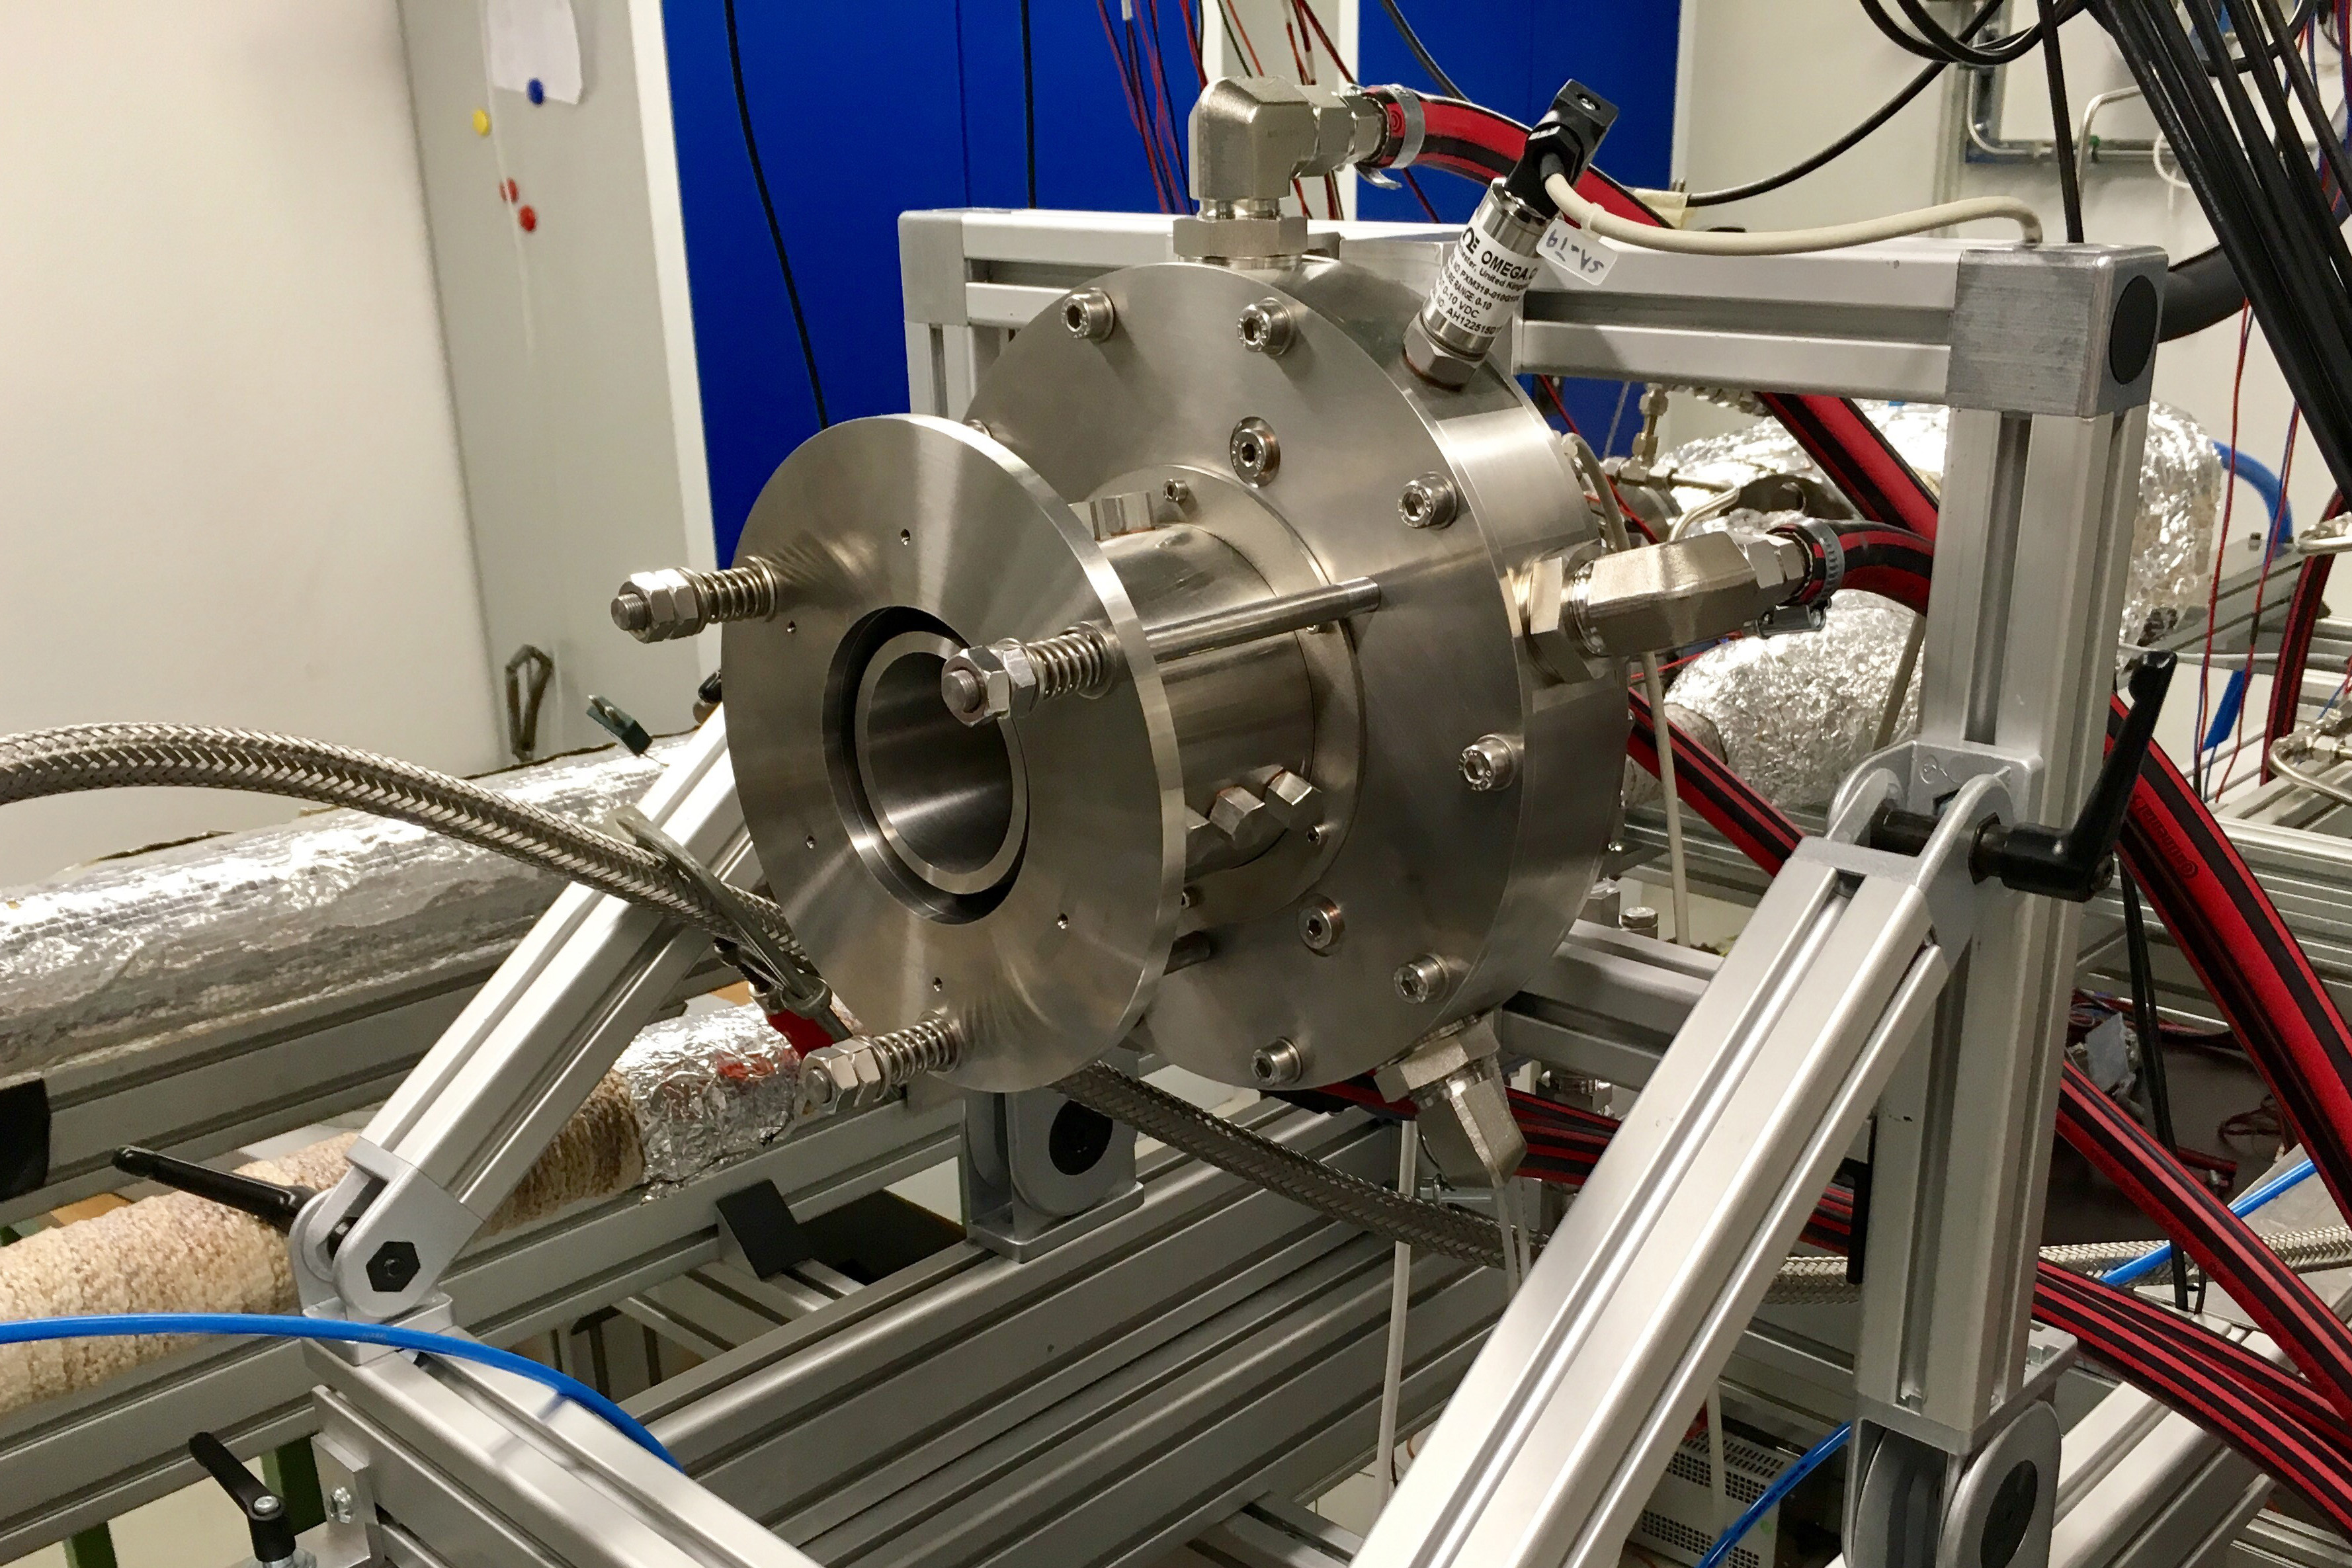
\includegraphics[width=0.825\textwidth]{./figures/test_stand_crop.jpg}
		\captionof{figure}{Experimental setup at TUB.}
		\label{fig:facility}
\end{minipage}
\end{figure}

% ------------------- begin table ------------------------
\newcolumntype{L}[1]{>{\raggedright\let\newline\\\arraybackslash\hspace{0pt}}m{#1}}
\newcolumntype{C}[1]{>{\centering\let\newline\\\arraybackslash\hspace{0pt}}m{#1}}
\newcolumntype{R}[1]{>{\raggedleft\let\newline\\\arraybackslash\hspace{0pt}}m{#1}}
\begin{table}[ht]
	\begin{center}
		\begin{threeparttable}
			\caption{RDC geometry at TUB}
			\label{tab:exp}
			\begin{tabular}{L{0.4\columnwidth} R{0.4\columnwidth}}
				
				Property							&(units)	\\		
				\hline
				Outer annulus diameter			&90~mm							\\
				Annulus width					&7.6 and 15~mm 					\\
				Air injection gap height			&1 and 1.6~mm					\\
				Air injection area				&282.7 and 452.4~$\mathrm{mm}^2$	\\
				Fuel injection hole diameter		&0.5~mm							\\
				Number of fuel injection holes	&100								\\
				Fuel injection area				&19.6~$\mathrm{mm}^2$			\\
				
			\end{tabular}
		\end{threeparttable}
	\end{center}
\end{table}
% ------------------- end table ---------------------------------------

%\begin{figure}[ht]
%	\centering
% 	\includegraphics[width=1\textwidth,trim=0 0 0 0,clip]{./figures/RDC_setup.pdf}
% 	\caption{Experimental setup at TUB}
% 	\label{fig:exp_setup}
%\end{figure}

The RDC test stand at TUB is currently being commissioned. The RDC is based on a design developed by Shank \cite{Shank2012}, and has previously been studied in combustion experiments at UC and as well as by other groups \cite{Naples2013, Paxson2015, Anand2016, St.George2015a, Driscoll2015, Pandiya2016}. The RDC design was modified to allow for operation initially at lower reactant flow rates than in its original design, while increasing its modularity. A cross-sectional view can be seen in Fig.~\ref{fig:exp_setup} with a radially inward oriented air/oxidizer supply and discrete fuel supply. Various reactant injection schemes can be implemented by changing the fuel and air injection plates. The modified design also allows for easy exchangeability of the RDC center body and outer body, enabling the operation with different fuels by altering the detonation annulus width $\Delta$. The outer body can also be exchanged for a quartz version to allow for optical access to the reaction zone.  The final design is shown in Fig.~\ref{fig:facility}, while Tab.~\ref{tab:exp} is detailing the main dimensions of the RDC. The RDC is equipped with multiple sensor ports, of which twelve are placed in the detonation annulus and distributed 120 degrees radially and along the axis of the chamber. Additional ports are radially distributed in the air injection gap to study pressure feedback into that zone, while the pressure and temperature in the supply plena are also monitored. The sensor ports are designed to accept a broad range of sensors, including pressure and ionization probes to study the detonation velocity and pressure distribution in and around the reaction zone. A mobile flow control system utilizing interchangeable sonic nozzles was designed and built for reactant supply to the RDC and is currently equipped for air flow rates up to $0.5$~kg/s and hydrogen flow rates up to 26~g/s.


\section{Current and Ongoing Results}

\begin{figure}[ht]
	\centering
 	\includegraphics[width=0.8\textwidth,trim=0 0 0 0,clip]{./figures/Phi_Levels_5hole.png}
 	\caption{Normalized fuel-to-air ratio for various blowing ratios along the longitudinal plane and several cross sections along the jet.}
 	\label{fig:JIC}
\end{figure}

During the initial design and development stages of the RDC test stand, a scaled model cross section of the RDC was built and implemented in the water tunnel at TUB in order to study the reactant mixing. A dye containing water jet issuing into a confined crossflow of water was studied by means of high speed PLIF. The model was scaled to maintain the Reynolds numbers, the momentum ratio and the blockage ratio of the crossflow by the jet (defined as the ratio of jet separation to jet diameter). Several different injection schemes were studied including variations of injection location and the momentum ratio. The results showed that the mixing quality is highly dependent on the jet-to-crossflow momentum ratio and whether the jet issues directly into the detonation annulus or if it is confined by the air injection gap. In Fig.~\ref{fig:JIC} the dye concentration was normalized by the individual perfectly premixed value. This normalization is denoted here as the Normalized Fuel-to-Air Ratio (NFAR) and is shown for various blowing ratios (a reduced form of the momentum ratio when the fluids have identical densities). Only the standard hole position is shown in this figure, however measurements were also conducted with the fuel injection advanced into the crossflow confinement. Measurements were made along the longitudinal plane of the jet as well as at several planes perpendicular to the longitudinal plane. From this we are able to observe the impact of the confinement geometry along with the blowing ratio on the quality of mixing of the fuel jets as well as the mixing in the interstitial region between the discrete jets. From Fig.~\ref{fig:JIC}, one can clearly see that at lower blowing ratios the jets remain as individual discrete fuel jets with minimal interaction between each other or mixing with the crossflow. Increasing the blowing ratio results in a much more rapid mixing of the jets with the crossflow fluid as well as spanning the interstitial space between the jets, resulting in a more homogeneous overall mixture. We are also able to observe through this and other campaigns that the mixing of the jet fluid is also impacted by the interaction of the jet with the shear layer formed by the crossflow separating from the corner of the crossflow confinement. From this we have observed that the quality of mixing can be controlled by the combination of the blowing ratio and the position of the fuel jet relative to the confinement. 

Based on these water tunnel studies, several different fuel and air injection strategies are currently undergoing development and testing. The primary focus of these studies is to understand the impact of fuel injection and impingement on the air injection confinement on the quality of mixing in the RDC and on extending the operational map of the combustor. As such, the operation of the engine will be tested with the fuel injection impinging and not impinging on the crossflow confinement. Additionally the position of the fuel injection holes will be advanced into the crossflow confinement allowing for variation in the blockage ratio of the jets and the separation of the jet-to-jet spacing.

\section{Conclusion}
A new research group concentrating on RDCs was established at Technische Universität Berlin, in collaboration with the University of Cincinnati. An RDC test stand was designed and developed and is currently being commissioned. The combined efforts of TUB and UC promise significant advancements in the field of PGC with the focus on thermally-managed RDC operation. The initial focus of this group is to investigate reactant mixing in the context of the RDC geometry. This has resulted in a two-pronged approach. During the development stages of the RDC, first investigations of reactant mixing in a scaled model RDC cross section in a water tunnel revealed the impact of several parameters on the mixing quality. From these results, it appears that the jet momentum ratio and position of the fuel jet relative to the air confinement are two powerful parameters in controlling mixing. Therefore, an improved and optimized mixing scheme is being investigated and implemented in an RDC and its impact on the operation will be studied.

\section*{Acknowledgments}
Financial support from the Einstein Foundation Berlin is gratefully acknowledged.

% -------------------------------------------------------------------------------------------------------------------
% Bibliography
\bibliographystyle{aiaa}
\bibliography{all_lit}

\end{document}

% - Release $Name:  $ -
